\documentclass[format=acmsmall, review=false, screen=true]{acmart}

\usepackage{booktabs} % For formal tables
\usepackage{multirow}
\usepackage{amsmath}
\usepackage{amssymb}

\usepackage{xr}
\externaldocument{article}

\usepackage[ruled]{algorithm2e} % For algorithms
\renewcommand{\algorithmcfname}{ALGORITHM}
\SetAlFnt{\small}
\SetAlCapFnt{\small}
\SetAlCapNameFnt{\small}
\SetAlCapHSkip{0pt}
\IncMargin{-\parindent}
\setcounter{tocdepth}{4}

\def\thesection{SI-M-\arabic{section}}
\def\thefigure{SI-M-\arabic{figure}}

% Metadata Information
\acmJournal{CSUR}
\acmVolume{0}
\acmNumber{0}
\acmArticle{0}
\acmYear{0}
\acmMonth{0}
\copyrightyear{2019}
%\acmArticleSeq{9}

% Copyright
%\setcopyright{acmcopyright}
% \setcopyright{acmlicensed}
\setcopyright{rightsretained}
%\setcopyright{usgov}
%\setcopyright{usgovmixed}
%\setcopyright{cagov}
%\setcopyright{cagovmixed}
\acmPrice{0.00}

% DOI
\acmDOI{0000001.0000001}

% Paper history
\received{XXXXX}
\received[revised]{XXXXX}
\received[accepted]{XXXXX}

% \newcommand{\massa}{{\large \textsc{mass}}}
% \newcommand{\mass}{{\large \textsc{mass}}}
% \newcommand{\figgus}{{\large \textsc{figgus}}}
\newcommand{\massa}{MASS}
\newcommand{\mass}{MASS}
\newcommand{\figgus}{MASS}
% Document starts
\begin{document}
% Title portion. Note the short title for running heads 
\title[Notes in music]{Organization of notes in music}  
\author{Renato Fabbri}
% \orcid{1234-5678-9012-3456}
\affiliation{%
  \institution{University of S\~ao Paulo}
  \department{Institute of Mathematics and Computer Sciences}
  \streetaddress{Avenida Trabalhador S\~ao Carlense, 400 - Centro}
  \city{S\~ao Carlos}
  \state{SP}
  \postcode{13566-590}
  \country{Brazil}}
\author{Vilson Vieira da Silva Junior}
\affiliation{%
  \institution{Cod.ai}
%  \department{Research and Development}
  \city{Berlin}
  \state{BE}
  \postcode{???}
  \country{DE}
}
\author{Ant\^onio Carlos Silvano Pessotti}
\affiliation{%
  \institution{Universidade Metodista de Piracicaba}
  \department{??}
  \city{Piracicaba}
  \state{SP}
  \postcode{???}
  \country{Brazil}}
\author{D\'ebora Cristina Corr\^ea}
\affiliation{%
  \institution{University of Western Australia}
  \department{??}
  \city{Piracicaba}
  \state{SP}
  \postcode{???}
  \country{AU}
  }
\author{Osvaldo N. Oliveira Jr.}
\affiliation{%
  \institution{University of S\~ao Paulo}
  \department{S\~ao Carlos Institute of Physics}
  \streetaddress{Avenida Trabalhador S\~ao Carlense, 400 - Centro}
  \city{S\~ao Carlos}
  \state{SP}
  \postcode{13566-590}
  \country{Brazil}
  }

\begin{abstract}
  This Supporting Information document holds an extension of the exposition in the main document to encompass canonical music theory, i.e. to bridge the procedures of synthesizing notes to the techniques of organizing them as music.
\end{abstract}

%
% The code below should be generated by the tool at
% http://dl.acm.org/ccs.cfm
% Please copy and paste the code instead of the example below. 
%
\begin{CCSXML}
  <ccs2012>
    <concept>
      <concept_id>10010405.10010469.10010475</concept_id>
      <concept_desc>Applied computing~Sound and music computing</concept_desc>
      <concept_significance>500</concept_significance>
    </concept>
    <concept>
      <concept_id>10010147.10010341.10010342.10010343</concept_id>
      <concept_desc>Computing methodologies~Modeling methodologies</concept_desc>
      <concept_significance>300</concept_significance>
    </concept>
    <concept>
      <concept_id>10002944.10011122.10002945</concept_id>
      <concept_desc>General and reference~Surveys and overviews</concept_desc>
      <concept_significance>300</concept_significance>
    </concept>
    <concept>
      <concept_id>10002944.10011122.10002946</concept_id>
      <concept_desc>General and reference~Reference works</concept_desc>
      <concept_significance>300</concept_significance>
    </concept>
  </ccs2012>
\end{CCSXML}

\ccsdesc[500]{Applied computing~Sound and music computing}
\ccsdesc[300]{Computing methodologies~Modeling methodologies}
\ccsdesc[300]{General and reference~Surveys and overviews}
\ccsdesc[300]{General and reference~Reference works}

%
% End generated code
%


\keywords{music, acoustics, psychophysics, digital audio, signal processing}


\thanks{This work is supported by FAPESP and CNPq.}


\maketitle

% The default list of authors is too long for headers}
\renewcommand{\shortauthors}{R. Fabbri et al.}


% \section{}\label{notasMusica} \label{sec:notesMusic}
\section*{Introduction}
Let $S=\left\{  s_j=T_i^j=\{t_i^j\}_{i=0}^{\Lambda_j-1} \right\}_{j=0}^{H-1}$ be a the sequence of $H$ musical events $s_j$.
Consider $S$ as a `musical structure'.
This section is dedicated to techniques that make $S$ interesting and enjoyable for hearing.
More specifically, what follows is a summary of academic music composition theory and praxis.
This section does not benefit from equations that dictate the amplitude of each sample as deeply as the previous sections.
Even so, we understand that this content is very useful for synthesizing music and is not trivially integrated to Sections~\ref{sec:discNote}
and~\ref{sec:varInternas}.
The concepts are given algorithmic implementations in \mass~\cite{massListings} and can be further formalized~\cite{topos},
although at a cost of prompt intelligibility which we chose to avoid in this exposition.
All relations described in this section are implemented in the file \texttt{src/sections/4.py}.
The musical pieces related to this section are on the directory~\texttt{src/pieces4/}.~\cite{MASSA}

The elements of $S$ can be overlapped by mixing them together, as in
Equation~\ref{eq:mixagem} and Figure~\ref{fig:mixagem}, for building intervals and chords. This reflects the `vertical thought' in music. On the other hand, the concatenation of events
in $S$, as in Equation~\ref{eq:concatenacao} and in Figure~\ref{fig:concatenacao},
yields melodic sequences and rhythms, which are associated with the `horizontal thought'.
The fundamental frequency $f$ and the starting moment
(attack) are generally considered the most important characteristics of the elements $s_j$.
These observations are convenient to describe and create music constituted by pitches and by temporal metrics and rhythms.
We will start by considering such aspects of musical organization as they are more
traditional in music theory and are usually easier to understand.

\section{Tuning, intervals, scales and chords}\label{subsec:afinacao}
\subsection{Tuning}
Doubling the frequency is equivalent to ascending one octave ($f=2f_0$).
The octave division in twelve pitches is the canon for classical western music.
Its usage has also been observed
outside western tradition, e.g. in ceremonial/religious and ethnic contexts~\cite{Wisnick}.
The intervals between the pitches need not to be equivalent,
as will become clear in the next paragraphs, but, roughly,
the factor given by $\varepsilon=2^{\frac{1}{12}}$ defines a semitone,
i.e. if $f=2^{\frac{1}{12}}f_0$, there is a semitone between
$f_0$ and $f$.
This entails a note grid along the spectrum in which, given a frequency $f$,
any other fundamental frequency $f'$ is related to $f$ by $f'= \varepsilon^i f$ where $i$ is an integer.
Twelve successive semitones yield an
octave.
Notice that equivalences of semitones and octaves are not absolute:
2 pitches related by an octave ($f_2 = 2f_1$) are different at least because one is higher than the other,
but are equivalent in the sense that they have similar uses and might be added or substituted
in a sound without introducing much novelty or change;
semitones might not be perceived as equivalent "distances"
(this is dependent on context and listener),
but are equivalent e.g. for transposing melodies, harmonies
and other pitch-related structures.

The absolute accuracy of $\varepsilon=2^\frac{1}{12}$ is usual in computational implementations.
Performances with real musical instruments, however, often present semitones that are not exactly $2^{\frac{1}{12}}$
because the pitches yield by such grid do not match the harmonics.
The fixed interval $\varepsilon=2^{\frac{1}{12}}$ characterizes an equally tempered tuning but there are other tunings. The first formalizations of tunings (that the scientific tradition has reported) date from around two thousand years before the advent of the equal temperament~\cite{Roederer}.
Two emblematic tunings are:
\begin{itemize}
    \item The {\bf just intonation}, defined by association of intervals with ratios of low-order integers, as found in the harmonic series. E.g. the white piano keys from C to C are achieved by the ratios of frequency: 1, 9/8, 5/4
    4/3, 3/2, 5/3, 15/8, 2/1. The semitone 16/15 is also often considered.
		There are many ways to perform the division of the 12 notes in the just intonation.
    \item The {\bf Pythagorean tuning}, based on the interval 3/2 (perfect fifth). The 'white piano keys' become: 1, 9/8, 81/64, 4/3, 3/2, 27/16, 243/128, 2/1. Also often used are the 'minor second' 256/243, the 'minor third' 32/27, the 'augmented fourth' 729/512, the 'diminished fifth' 1024/729, the 'minor sixth' 128/81 and the 'minor seventh' 16/9. 
\end{itemize}

In order to account for micro-tonality\footnote{Micro-tonality is the use of intervals smaller
than one semitone and has ornamental and structuring functionalities in music. The division of the octave in $12$ notes has physical grounds but is still a \emph{convention} adopted by western classical music. Other tunings are incident, e.g. a traditional Thai music style uses an octave division in seven notes equally spaced ($\varepsilon=2^{\frac{1}{7}}$),
which allows intervals quite different than those found when $\varepsilon=2^{\frac{1}{12}}$~\cite{Wisnick}.}, non-integer values can be used as factors of $\varepsilon=2^{\frac{1}{12}}$ between frequencies, or one can maintain the usage of integer values and change $\varepsilon$. For example, a tuning that approximates the harmonic series
is proposed with the equal division of the octave in $53$ notes:
$\varepsilon=2^{\frac{1}{53}}$~\cite{microtonalidade}.
Note that if $S=\{s_i\}$ is a pitch sequence related by means of $\varepsilon=2^{1/\eta}$, the sequence $S'$ with the same notes, but related by $\varepsilon'=2^{1/\eta'}$, is 
$S'=\left\{s_i'\right\}=\left\{
s_i \frac{\eta'}{\eta}\right\}$ because:

\begin{equation}\label{eq:micro}
\begin{split}
    F   & = \{f_i\}\\
    S   & = \{s_i\} \Rightarrow f_i = f 2^{s_i/\eta}\\
    S'  & = \{s'_i\} \Rightarrow f_i = f 2^{s'_i/\eta'}\\
    f_i & =  f 2^{s_i/\eta} = f 2^{s'_i/\eta'} \Rightarrow s'_i = s_i\frac{\eta'}{\eta} 
\end{split}
\end{equation}

The music piece \emph{Micro
tone} exemplifies the use of microtonal features.

\subsection{Intervals}\label{subsec:intervalos}
Using the ratio $\varepsilon=2^{\frac{1}{12}}$ between note frequencies (i.e.\ one semitone)
the intervals in the twelve tone system can be represented by integers. Table~\ref{eq:intervalos} summarizes the intervals: traditional notation, qualifications of consonance and
dissonances, and number of semitones.

\begin{table*}[htp!]
\centering
    \caption{Musical intervals: traditional notation, basic classification for dissonances and consonances, and number of semitones. Unison, fifth and octave are the perfect (P) consonances. Major (M) and minor (m) thirds and sixths are the imperfect consonances. Minor seconds and major sevenths are the harsh (also strong or sharp) dissonances. Major seconds and minor sevenths are the mild (also weak) dissonances. Perfect fourth is a special case, as it is a perfect consonance when considered as an inversion of the perfect fifth and a dissonance or an imperfect consonance otherwise. Another special case is the tritone (A4 or aug4, d5 or dim5, tri or TT). This interval is consonant in some cultures.
	For tonal music, the tritone indicates a dominant (chord, function or harmonic field, see Section~\ref{subsec:harmonia}) and seeks urgent resolution into a third or sixth, and due to this instability it is considered a dissonant interval.}
\begin{tabular}{ c | c | c }\hline
    \multicolumn{3}{c}{\bf consonances}  \\\hline
   & traditional notation & number of semitones \\
   perfect: & P1, P5, P8 & 0, 7, 12 \\
 imperfect: & m3, M3, m6, M6 & 3, 4, 8, 9 \\\hline\hline
    \multicolumn{3}{c}{\bf dissonances} \\\hline
 & traditional notation & number of semitones \\
 strong: & m2, M7 & 1, 11 \\
 weak: & M2, m7 & 2, 10 \\\hline\hline
    \multicolumn{3}{c}{\bf special cases} \\\hline
 & traditional notation & number of semitones \\
 consonance or dissonance: & P4 & 5 \\
 dissonance in Western tradition: & tritone, aug4, dim5 & 6 \\\hline
\end{tabular}\label{eq:intervalos}
\end{table*}

The nomenclature, based on conveniences for tonal music and practical aspects of manipulating notes, can be specified
as follows~\cite{Roederer,Wisnick}:

\begin{itemize}
    \item Intervals are inspected first by the number of steps between notes. The simple intervals (which are at most an octave wide) are: first (unison), second, third, fourth, fifth, sixth, seventh and eighth (octave).
		Each of these intervals are related to one step less the their names suggest: a third is an interval with two steps.
		As can be noticed in Table~\ref{eq:intervalos}, one step is not one semitone.
		A step, in this sense, is yield by two consecutive notes in a musical scale.
		A scale for now can be regarded as any arbitrary monotonic sequence of pitches and will be discussed in the next section.
            \item The intervals are represented by numeric digits, e.g. 1, 3, 5 are a unison, a third and a fifth, respectively\footnote{Integers might also be used to express the number of semitones in an interval.}.
	\item An interval wider than an octave (e.g. ninth, tenth, eleventh) is called a 'compound interval' and is classified in terms of the simple interval between the same notes but in the same octave. Their notation can be achieved by adding a multiple of
                7 to the simple interval: P11 is an octave plus a forth ($7 + P4 = P11$), M9 is an octave plus a major second ($7 + M2 = M9$),
                m16 is two octaves and a minor second ( $2\times 7 + m2 = m16$).
	\item Quality of each interval: perfect consonances --
                i.e.\ unison, fourth, fifth and octave -- are 'perfect'. The imperfect consonances -- i.e.\ thirds and sixths -- and dissonances -- i.e.\ seconds and sevenths -- can be major and minor. The tritone is an exception to this rule because it is a dissonant interval and cannot be major or minor.
	\item The perfect fourth can be a perfect consonance or a dissonance according to the context and theoretical background. As a general rule, it can be considered a consonance except when it is followed by a third or a fifth by the movement of the notes.
	\item The tritone is a dissonance in Western music because
		it is typical of the ``dominant'' chord (see Section~\ref{subsec:harmonia}) and represents (or yields) instability.
                Some cultures consider the interval a consonance and use it as a stable interval.
	\item A major interval decreased by one semitone results in a minor interval. A minor interval increased by one semitone results in a major interval.
	\item A perfect interval (P1, P4, P5, or P8), or a major interval (M2, M3, M6 or M7), increased
by one semitone results in an augmented interval (e.g.\
aug3 has five semitones). The augmented forth
is also called tritone (aug4, tri, or TT).
	\item A perfect interval or a minor interval (m2, m3, m6 or m7), decreased by one semitone results in a diminished interval. The
diminished fifth is also called tritone (dim5, tri, or TT).

	\item An augmented interval increased by one semitone results in a `doubly-augmented' interval; a diminished interval decreased by one semitone results in a `doubly-diminished' interval.
	\item Notes played simultaneously yield a harmonic interval.
	\item Notes played as a sequence in time yield a
                melodic interval.  When the lowest note comes first there is an ascending interval, while a descending interval is observed when the highest note comes first. 
	\item A simple interval is inverted if the lowest pitch is raised one octave, or if
                the highest pitch is lowered one octave. The sum of an interval and its inversion is
                9 (e.g.\ m7 is inverted to M2: $m7+M2=9$). An inverted major
                interval results in a minor interval and vice-versa. An
                inverted augmented interval results in a diminished interval
                and vice-versa (inverting a doubly-augmented results in a
                doubly-diminished and vice-versa, etc).
                An inverted perfect interval is a perfect interval as well.
\end{itemize}

The augmented/diminished intervals and the doubly-augmented/doubly-diminished intervals have the same number of semitones of other intervals (e.g. minor, major or perfect) and are consequences of the tonal system.
Scale notes are in fact different pitches, with specific uses and functions. Henceforth, in a \textit{C flat} major scale, the tonic -- first degree -- is \textit{C flat}, not \textit{B}, and the leading tone -- seventh degree -- is \textit{B flat}, not \textit{A sharp} or \textit{C double flat}.
To grasp what this entails for intervals, let the second degree (second note) of a scale be one semitone from the first degree. Consider also the leading tone (i.e. the seventh degree at one ascending semitone from the first degree). There is a diminished third between the seventh and second scale degrees~\cite{Lacerda}.
Notice that the dim3 is only two semitones wide, as is the major second (or e.g. an doubly-augmented unisson!).

This description summarizes the traditional nomenclature (or theory) of musical intervals~\cite{Lacerda}.
The music piece \emph{Intervals} explores these intervals in both independent and interrelated ways~\cite{MASSA}.

\subsection{Scales}\label{subsec:escalas}
A scale is an ordered set of pitches. Strictly speaking, any (ordered) set of pitches can be considered a scale. The complexity of musical scales lean mostly on tradition, i.e. on the scales and their uses which result from practice throughout history. Usually, scales repeat at each octave. The ascending sequence with all notes from the octave division in 12 equal intervals ($\varepsilon=2^{\frac{1}{12}}$) is known as the chromatic scale within the equal temperament. There are 5 perfectly symmetric divisions of the octave using the chromatic scale. These divisions are often regarded as scales themselves owing to the easy and peculiar uses they entail.

Let $e_i$ be integers indexed by $i$ such that
$f=\varepsilon^{e_i} f_0$,
where $f_0$ is any fixed frequency.
The symmetric scales mentioned above can be expressed as:
\begin{equation}\label{escSim}
\begin{aligned}
	\text{chromatic}    & = E^c    & = \{e_i^c\}_0^{11}   & =  \{0,1,2,3,4,5,6,7,8,9,10,11\} & = \{i\}_0^{11}\\
	\text{whole tones}  & = E^{wt} & = \{e_i^{wt}\}_0^{5} & = \{0,2,4,6,8,10\}               & = \{2i\}_0^{5} \\
	\text{minor thirds} & = E^{mt} & = \{e_i^{mt}\}_0^{3} & = \{0,3,6,9\}                    & = \{3i\}_0^3 \\
	\text{major thirds} & = E^{Mt} & = \{e_i^{Mt}\}_0^{2} & = \{0,4,8\}                      & = \{4i\}_0^2\\
	\text{tritones}     & = E^{tt} & = \{e_i^{tt}\}_0^{1} & = \{ 0, 6 \}                     & = \{6i\}_0^1
\end{aligned}
\end{equation}

For example, the third note of the whole tone scale with $f_0=200Hz$ is $f_3=\varepsilon^{e_2^{wt}}.
f_0 = 2^{\frac{4}{12}} .
200 \approxeq 251.98
Hz$.
These `scales', or patterns, generate stable structures by their internal symmetries and can be repeated in a sustained way which is musically effective.
Section~\ref{estCic} discusses other aspects of symmetries in music.
The musical piece \emph{Crystals} uses each one of these scales, in both melodic and harmonic constructions.

The \emph{diatonic scales} have seven notes in which the consecutive intervals include five whole tones\footnote{A (whole) tone is an interval that is two semitones wide: $f'=2^{\frac{2}{12}}f$.} and two semitones (in each octave). There are seven of them:

\begin{equation}\label{eq:escalas}
\begin{aligned}
	\text{aeolian}    & = \text{natural minor scale}  & = & \\
			  & = E^m = \{e_i^m\}_0^6       & = & \{0,2,3,5,7,8,10\} \\
	\text{locrian}    & = E^{lo} = \{e_i^{lo}\}_0^6 & = & \{0,1,3,5,6,8,10\} \\ 
	\text{ionian}     & = \text{major scale}          & = &  \\
			  & = E^M = \{e_i^M\}_0^6       & = & \{0,2,4,5,7,9,11\} \\
	\text{dorian}     & = E^{d} = \{e_i^{d}\}_0^6   & = & \{0,2,3,5,7,9,10\} \\
	\text{phrygian}   & = E^{p} = \{e_i^{p}\}_0^6   & = & \{0,1,3,5,7,8,10\} \\
	\text{lydian}     & = E^{l}=\{e_i^{l}\}_0^6     & = & \{0,2,4,6,7,9,11\} \\
	\text{mixolydian} & = E^{mi} = \{e_i^{mi}\}_0^6 & = & \{0,2,4,5,7,9,10\}
\end{aligned}
\end{equation}

\noindent They have only major, minor and perfect intervals.
The unique exception is the tritone found as an augmented fourth or a diminished fifth.
% It is useful to name the diatonic scale degrees as: tonic, supertonic, mediant, subdominant, dominant, submediant, leading note (and then the tonic again).
% Accordingly, the first degree is the tonic, the fifth degree is the dominant.
% These names are unanimously used for the major scale and within tonal harmony (as presented in Section~\ref{subsec:harmonia}.
% In other scales these names might be used by extension.
% One critical exception is the dominant in the locrian scale: it is not a perfect fifth above the tonic, so it does not play the same role as in the other scales.
% This is the main reason why the locrian is sometimes not considered a diatonic scale.
Diatonic scales follow a circular pattern of successive intervals \textit{tone, tone, semitone, tone, tone, tone, semitone}. Thus, it is possible to write:

\begin{equation}\label{eq:relacaoDia}
\begin{split}
\{d_i\} & =\{2,2,1,2,2,2,1\} \\
e_0 & =0 \\
e_i & =d_{(i+\kappa)\%7}+e_{i-1} \quad for \;\;  i > 0
\end{split}
\end{equation}

\noindent with $\kappa \in \mathbb{N}$. For each mode (of Equations~\ref{eq:escalas}) there is only one $\kappa \in [0,6]$ for which $\{e_i\}$ (of Equations~\ref{eq:relacaoDia}) matches. 
For example, a brief inspection reveals that
$e_i^{l}=d_{(i+2)\%7}+e_{i-1}^{l}$. Thus, $\kappa=2$ for the lydian scale.

The minor scale have two additional forms, named harmonic and melodic:

\begin{equation}\label{eq:escalasMenores}
\begin{split}
\text{natural minor}&  = E^m = \{e_i^m\}_0^6 = \\
                                           &  = \{0,2,3,5,7,8,10\} \\
\text{harmonic minor}                      &  = E^{mh} = \{e_i^{mh}\}_0^6 = \\
                                           &  = \{0,2,3,5,7,8,11\} \\
\text{melodic minor}                       &  = E^{mm} = \{e_i^{mm}\}_0^{14} = \\
                                           &  = \{0,2,3,5,7,9,11,12,10,8,7,5,3,2,0\} \\
\end{split}
\end{equation}

The different ascending and descending contours of the melodic minor scale is required in tonal music.
The minor scale has one whole tone between the seventh and eigth (or first) degrees but
the separation by one semitone is critical to the polarization of the first degree.
This is not necessary in the descending trajectory, and therefore the scale recovers the standard form.
The harmonic scale presents the modified seventh degree but does not avoid the augmented second between the sixth and seventh degrees; it does not consider the melodic trajectory and thus does not need to avoid the aug2~\cite{Harmonia}.

Although it is not a traditional scale, the harmonic series is often used as such:
\begin{equation}\label{eq:serieHarmonica}
\begin{split}
H = & \{h_i\}_0^{19}= \\
    =  & \{ 0,12,19+0.02,  24,28-0.14, 31+0.2, 34-0.31, \\
                     & 36, 38+0.04,40-0.14, 42-0.49, 43+0.02, \\
                     & 44+0.41, 46-0.31, 47-0.12, \\
                     & 48, 49+0.05, 50+0.04, 51-0.02, 52-0.14   \}
\end{split}
\end{equation}

In this scale, the frequency of the $i$th note $h_i$ is the frequency of $i$th harmonic $f_i=\varepsilon^{h_i} f_0$ from the spectrum generated by $f_0$. Natural sounds have such frequencies (as discussed in Section~\ref{sec:discNote}) usually with deviations from the expected values and with noise.

Many other scales can be expressed using the framework exposed in this section, e.g. the pentatonic scales and the modes of limited transposition of Messiaen~\cite{Messiaen}.

One last observation: the words \emph{scale} and \emph{mode} are often used as synonyms both in the literature and in colloquial discussions.
The word \emph{mode} can also be used to mean two other things:
\begin{itemize}
	\item an unordered set of pitches (i.e. an unordered scale).
	\item A scale used in the context of modal harmony, in the sense presented in Section~\ref{subsec:harmonia}.
\end{itemize}

\subsection{Chords}\label{subsec:acordes}
A musical chord is implied by the simultaneous occurrence of three or more notes. Chords are often based on triads, especially in tonal music. Triads are built by two successive thirds
within 3 notes: root, third and fifth. If the lower note of a chord is the root, the chord is in the root position, otherwise it is an inverted chord. A closed position is any in which no chord note fits between two consecutive
notes~\cite{Lacerda}, any non-closed position is an open position. In closed and fundamental positions,
and with the fundamental denoted by $0$, triads can be expressed as:
\begin{equation}\label{triades}
\begin{split}
\text{major triad} = A^M= \{a_i^M\}_0^2=\{0,4,7\} \\ 
\text{minor triad} = A^m = \{a_i^m\}_0^2=\{0,3,7\} \\
\text{diminished triad} = A^d = \{a_i^d\}_0^2=\{0,3,6\} \\
\text{augmented triad} = A^a = \{a_i^a\}_0^2=\{0,4,8\}
\end{split}
\end{equation}

It is commonplace to consider another successive third: it is sufficient to include $10$ as the highest note to achieve a tetrad with a minor seventh, or include $11$ in order to achieve a tetrad with a major
seventh. Inversions and open positions can be obtained with the 
addition of $\pm 12$ to the selected note. Incomplete triadic chords, with extra notes ('dirty' chords), and non-triadic
are also common.
These are often interpreted as the result of further extending the succession of thirds.
E.g. $\{0,2,4,7\}$ will often be understood as a major chord with a major ninth (a major ninth has 14 semitones and $14-12 = 2$).

For general guidance:
\begin{itemize}
        \item A fifth confirms the root (fundamental).
		There are theoretical discussions about why this happens, and the most usual arguments are that the fifth is the first (non-octave) harmonic of a note and that the harmonics of the fifth are in the harmonics of the fundamental.
                Important here is to grasp the fact that musical theory and practice assures that the fifth establishes (or helps to establish) the fundamental as the root of a chord.
        \item Major or minor thirds from the root entails major or minor chord qualities.
        \item Every tritone, especially if built between a major third and a minor seventh, tends to resolve into a third or a sixth.
        \item Note duplication is avoided. If duplication is needed, the preference is, in descending order: the root, fifth, third and seventh.
        \item Note omission is avoided in the triad. If needed, the fifth is first considered for omission, then third and then the fundamental.
        \item It is possible to build chords with notes different from triads, particularly if they obey a recurrent logic or sequence that justifies these different notes.
        \item Chords built by successive intervals different from thirds -- such as fourths and seconds -- are recurrent in compositions of advanced tonalism or experimental music.
        \item The repetition of chord successions (or of characteristics they hold) fixes a trajectory and makes it possible to 
introduce exotic arrangements without implying in musical incoherence.
\end{itemize}

\section{Atonal and tonal harmonies, harmonic expansion and modulation}\label{subsec:harmonia}
Omission of basic tonal structures is the key to achieving modal and atonal harmonies. In the absence of minimal tonal organization,
harmony is (usually) considered modal if the notes match some diatonic scale (see Equations~\ref{eq:escalas}) or if there is only a small number of notes. If basic tonal progressions are absent and notes do not match any diatonic scale and are sufficiently diverse and dissonant (between themselves) to avoid reduction of the notes by polarization\footnote{By polarization we mean having some notes that are way more important than others and to which the other notes are ornaments or subordinates.}, the harmony is atonal. In this classification, the modal harmony is not tonal or atonal and is reduced to the incidence of notes within a (most often diatonic) scale and to the absence of tonal structures. Following this conceptualization, one observes that atonal harmony is hard to be realized and, indeed, no matter how dissonant and diverse
a set of notes is, tonal harmonies arise very easily if not avoided laboriously~\cite{harmEXT}.

\subsection{Atonal harmony}\label{sec:atonal}
In fact, atonal music techniques avoid that a direct relation of the notes with modes and tonality be established. Manifesting such atonal structures is of such difficulty that the dodecafonism emerged. Dodecafonism consists in the use a set of notes (ideally 12 notes) and the execution of each note, one by one, in the same
order. In this context, the tonic becomes difficult to be established. Nevertheless, the western listener automatically searches for tonal elements in music and obstinately finds them by unexpected and tortuous paths. The use of dissonant intervals (especially tritones) without resolution reinforces the absence of tonality. In this context, while creating a musical
piece, it is allowed:
\begin{itemize}
     \item To repeat pitches. By considering immediate repetition as an extension of the previous incidence, the use of the same pitch in sequence does not add relevant information.
     \item To play adjacent pitches (e.g. of a dodecafonic progression) at the same time, making harmonic intervals and chords.
     \item Use durations and pauses with freedom, respecting pitch order.
     \item Vary note sequences by temporal magnification and translation; or pitch transposition and sequence inversion, retrograde and retrograde inversion. See Sections~\ref{subsec:motivos} and~\ref{subsec:usosmusicais3} or specialized literature (such as ~\cite{serial}) for what these terms mean.
     \item Make variations in orchestration, articulation, spatialization, among other possibilities in presenting the same notes.
\end{itemize}

The atonal harmony can be observed, paradigmatically, within these presented conditions (which is a simple dodecaphonic model). Most of what was written by great dodecafonic composers,
e.g. Alban Berg and even Schoenberg, had the purpose of mixing tonal and atonal techniques.
Most frequently, atonal music is not strictly dodecafonic, but "serial",
i.e. they use the same kind of techniques based in (arbitrary) sequences (called the series or row)
of pitches and other sonic characteristics.

\subsection{Tonal harmony}
In the XX century, music with emphasis on sonorities/timbres, and rhythm, extended the concepts of tonality and harmony. Even so, tonal harmony is very often in artistic movements and commercial venues. In addition, dodecafonism itself is sometimes considered of tonal nature because it was conceived to deny tonal characteristics of polarization, i.e. it is based on tonalism.
In tonal or modal music, chords -- like the ones listed in
Equations~\ref{triades} -- built with the root at each degree of a scale (as listed in Equations~\ref{eq:escalas}) form the pillars of harmony.
Tonal (and modal) harmony deals with chord formation and progressions.
Even a monophonic melody entails harmonic fields, making it possible to perceive the chord progression even in unaccompanied melodies.

In the traditional tonal music, a scale has its tonic (first
degree) on any note, and can be major (with the same notes of the Ionian mode) or minor (same notes of the Eolian mode, the 'natural minor', which has both harmonic and melodic versions, as in Equations~\ref{eq:escalasMenores}). The
scale is the base for triads, each with its root in a degree: $\hat{1},\hat{2},\hat{3},\hat{4},\hat{5},\hat{6},\hat{7}$.
To build triads, the third and the fifth notes above the root are considered together with the root (or fundamental).
$\hat{1},\hat{3},\hat{5}$ is the first degree chord,
 built on top of the scale's first degree and central for tonal music. The chords of the fifth degree $\hat{5},\hat{7},\hat{2}$ ($\hat{7}$ sharp when in a minor scale) and of the forth degree $\hat{4},\hat{6},\hat{1}$ are also important.
 The triads built on the other degrees are less important then these and are usually understood in relation to them. The `traditional harmony' comprises conventions and stylistic techniques to create progressions with such chords~\cite{Harmonia}. 

The `functional harmony' ascribes functions to the three main chords and describes their use by means of these functions. The chord built on top of the first degree is the \textbf{tonic} chord (\textit{T} or \textit{t} for a major or minor tonic, respectively) and its function (role) consists on maintaining a center, usually referred to as a ``ground'' for the music. The chord built on the fifth degree is the \textbf{dominant} (\textit{D}, the dominant is always major) and its function is to lean for the tonic
(the dominant chord asks for a conclusion and this conclusion is the tonic). Thus, the dominant chord guides the music to the tonic. The triad built on the fourth degree is the \textbf{subdominant} (\textit{S} or \textit{s} for a major or minor
subdominant, respectively) and its function is to deviate the music from the tonic.
The tonal discourse aims at confirming the tonic using the tonic-dominant-tonic progression
which is expanded by using other chords in various ways.

The remaining triads are associated to these three most important chords. In the major scale, the associated relative (relative tonic \textit{Tr}, relative
subdominant \textit{Sr} and relative dominant \textit{Dr}) is the triad built a third below, and the associated counter-relative (counter-relative tonic \textit{Tc}, counter-relative subdominant \textit{Sc} and the counter-relative dominant \textit{Dc}) is the triad built in a third above. In the minor scale the same happens, but the triad a third below is called counter-relative (tC, sC) and the triad a third above is called relative (tR,
sR). The precise functions and musical effects of these chords are
controversial but are basically the same as the chords they are associated to.
Table~\ref{tab:harmonia} shows relations between the triads built at each degree of the major scale.

\begin{table}[htp!]
\centering
\caption{Summary of tonal harmonic functions on the major scale.
Tonic is the musical center, the dominant leans to the tonic and the subdominant moves the music away from
the tonic. The three chords can, in principle, be replaced by their
respective relative or counter-relative.}
\begin{tabular}{l | c | r}
relative & main chord of the function & counter-relative \\\hline\hline
$\hat{6},\hat{1},\hat{3}$ & tonic:       $\hat{1},\hat{3},\hat{5}$ & $\hat{3}, \hat{5},      \hat{7}$ \\
$\hat{3},\hat{5},\hat{7}$ & dominant:    $\hat{5},\hat{7},\hat{2}$ & [ $\hat{7},\hat{2},\hat{4}\#$ ] \\
$\hat{2},\hat{4},\hat{6}$ & subdominant: $\hat{4},\hat{6},\hat{1}$ & $\hat{6},\hat{1},       \hat{3}$
\end{tabular}
\label{tab:harmonia}
\end{table}

The dominant counter-relative should form a minor chord. It explains the change in the forth degree by a semitone above $\hat{4}\#$. The diminished chord
$\hat{7},\hat{2},\hat{4}$, is generally considered a `dominant seventh chord with the root omitted'~\cite{Koellheuteur}.
In the minor mode, there is a change in $\hat{7}$ by an ascending semitone to achieve a separation between $\hat{7}$ and $\hat{1}$ of a semitone. This is important for the dominant function (which should lean to the tonic). In this way, the dominant is always major, for both major and minor scales and, therefore, in a minor scale the relative dominant remains a third below, and the counter-relative remains a third above.

\subsection{Tonal expansion: individual functions and chromatic mediants}
Each chord can be stressed and developed by performing their individual dominant or subdominant, which are the triads based
on a fifth above or a fifth below, respectively. These individual dominants and subdominants,
in the same way, have also subdominants and dominants of their own. Given a tonality, any chord can occur, no matter
how distant it is from the most basic chords and from the notes of the scale.
The unique (theoretical) condition is that the occurrence presents a coherent trajectory of dominants and subdominants (or their relatives and counter-relatives) to the original tonality.

There are four mediants for each chord,
they are a third apart from the original chord and are simple triads,
as are the relatives and counter-relatives,
but retain the major/minor quality of the reference chord.
The
'chromatic mediants'
are the upper mediant, formed with the root at the third of the original chord;
and the lower mediant, formed by the fifth at the third of the original chord.
If two chromatic alterations exist, i.e.\ two notes are altered by one semitone,
it is a 'doubly-chromatic mediant'.
Again, there are two forms: 
the upper form, with a third in the fifth of the original triad; and the lower form, with a third in the root
of the original triad.
This relation between chords is considered of advanced tonalism, sometimes even considered as an expansion and dissolution of tonalism,
with strong and impressive effects although they are simple, consonant major/minor triads.
Chromatic mediants are used since the end of Romanticism by Wagner, Lizt, Richard Strauss, among others~\cite{Harmonia,Salzer}. 


\subsection{Modulation}
Modulation is the change of key (tonic, or tonal center) in music, being characterized by start and end keys, and transition artifacts.
Keys are always (thought of as) related by fifths and their relatives and counter-relatives. Some ways to perform modulation include:

\begin{itemize}
    \item Transposing the discourse to a new key, without any preparation. It is a common Baroque procedure and also incident in other periods. Sometimes it is 
    called phrasal modulation or unprepared modulation.
    \item Careful use of an individual dominant, and perhaps also the individual
    subdominant, to confirm change in key and harmonic field.
    \item Use of chromatic alterations to reach a chord in the new key by starting from a chord in the previous key. Called chromatic modulation.
    \item Featuring a unique note, possibly repeated or suspended with no accompaniment, common to start and end keys, it constitutes a peculiar way
    to introduce the new harmonic field.
    \item Changing the function, without changing the notes, of a chord.
        This procedure is called enharmony.
    \item Maintaining the tonal center and changing the key quality from major to minor
    (or vice-versa) is a `parallel modulation'. Keys with same tonic but
		different (major/minor) qualities are known as homonyms.
\end{itemize}

The dominant has great importance and is a natural pivot in modulations,
a fact that leads to the circle of fifths~\cite{Harmonia,Salzer,Koellheuteur,Harmony}.
Other inventive ways to modulate are possible, to point but one common example, the minor thirds tetrad ($E_i^{tm}$ in Equations~\ref{escSim}) can be sustained to bridge between tonalities, with the facility that both its tritones can be resolved in a number of ways.
The music piece \emph{Acorde cedo} explores these chord relations~\cite{MASSA}.

\section{Counterpoint}\label{subsec:contraponto}
Counterpoint is a set of techniques for the conduction of simultaneous melodic lines, or ``voices''.
The bibliography covers systematic ways to conduct voices, leading to scholastic genres like canons, inventions and fugues~\cite{Fux,SchoenbergContra}. It is possible to
summarize the rules of scholastic counterpoint, and it is known that Beethoven --
among others -- also outlined such a digest of counterpoint.

\begin{figure}[h!]
    \centering
        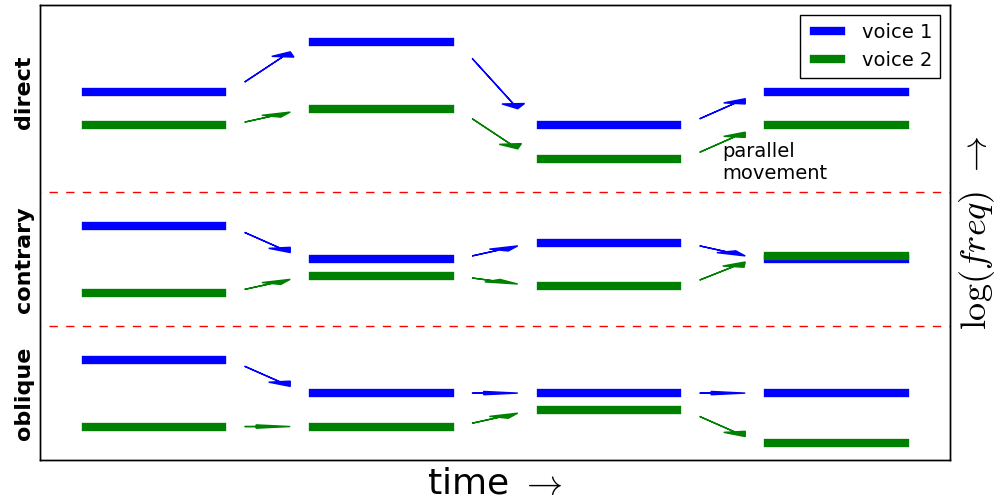
\includegraphics[width=.8\columnwidth]{figures/movContraponto_}
    \caption{Different motions of counterpoint aiming to preserve independence
        between voices. There are 3 types of motion: direct, contrary and
        oblique. The parallel motion is a type of direct motion.
	A voice is often called a 'melodic line' or a melody.}
        \label{fig:movContraponto}
\end{figure}

The main purpose of (scholastic) counterpoint is to conduct voices in a way that they sound independent.
In order to do that, the relative motion of voices (in pairs) is crucial and
categorized as: direct, oblique and contrary, as depicted in Figure~\ref{fig:movContraponto}.
The parallel motion is a direct motion in which the starting and final intervals are the same.
The golden rule here is to be careful with the direct motions, avoiding them
when ending in a perfect consonance.
The parallel motion should occur only between
imperfect consonances and no more than three consecutive times.
Dissonances can be forbidden or used only when followed and preceded by consonances of neighbor
degrees, i.e.\ adjacent notes in a scale.
The motions that lead to a
neighbor note in the scale sound coherent and are prioritized.
When having 3 or more voices, the melodic
relevance lies mainly in the highest and then in the lowest of the voices~\cite{Fux,Tragtenberg,SchoenbergContra}.

These rules were used in the musical piece \emph{Count point}~\cite{MASSA}.

\section{Rhythm}\label{subsec:ritmo}
\begin{table*}[htp!]
\caption{Durations heard as rhythm, as pitch and the transition.}
\begin{tabular}{  l | r r r r   r r r    r r r || r r  } \hline
& \multicolumn{10}{c}{\bf perception of durations as rhythm} & \multicolumn{2}{c}{}  \\
	duration (s) & \multirow{2}{*}{\bf ...}     & {\bf 32,}     & {\bf 16,}   & {\bf 8,}  & {\bf 4,}   & {\bf 2,}   & {\bf 1,}   & {\bf 1/2,} & {\bf 1/4,} & {\bf 1/8,} & \multirow{2}{*}{ ... transition } & \\
frequency (Hz) & & {\color{gray} 1/32,}   & {\color{gray} 1/16,} & {\color{gray} 1/8,} & {\color{gray} 1/4,} & {\color{gray} 1/2,} &  {\color{gray} 1,}  & {\color{gray} 2,}   & {\color{gray} 4,}   & {\color{gray} 8,} & & \\
& \multicolumn{10}{c}{ - } & \multicolumn{2}{c}{} \\ \hline
\end{tabular}
\vspace{.2cm}

	\begin{tabular}{  l | p{1.7cm}  || r r || r } \hline
& \multicolumn{1}{c}{} & \multicolumn{2}{c}{transition} &  \\
duration (s) & \multirow{2}{*}{\bf rhythm ...} & $\frac{1}{16}=62.5ms$ , & $\frac{1}{20}=50ms$ & \multirow{2}{*}{\bf ... pitch} \\
frequency (Hz) & & 16, & 20 &  \\
& \multicolumn{1}{c}{} & \multicolumn{2}{c}{transition} & \\ \hline
\end{tabular}
\hspace{3.36cm}
\vspace{.2cm}

	\begin{tabular}{  l | p{1.7cm} || r r r r r r }\hline
& \multicolumn{1}{c}{} &  \\
	duration (s) & \multirow{2}{*}{transition ...} & {\color{gray} 1/40} & {\color{gray} 1/80  } & {\color{gray} 1/160 } & {\color{gray} 1/320 } & {\color{gray} 1/640 } & \multirow{2}{*}{\bf ... } \\
frequency (Hz) & & {\bf 40}   & {\bf 80}   & {\bf 160}   & {\bf 320}   & {\bf 640}   & \\
& \multicolumn{1}{c}{} & \multicolumn{6}{c}{\bf perception of durations as pitch} \\ \hline
\end{tabular}
\hspace{2.70cm}
\label{tab:duracoes}
\end{table*}

Rhythmic notion is dependent on events separated by durations~\cite{Lacerda}.
Such events can be heard individually if their onsets are spaced by at least $50-63ms$.
For the temporal separation between them to be perceived as a duration,
the period should be even a bit larger, around $100ms$~\cite{microsound}.
It is possible to summarize the durations heard as rhythm or pitch
as in Table~\ref{tab:duracoes}~\cite{Alfaix, microsound}.

The transition span in Table~\ref{tab:duracoes} is minimized because the limits
are not well defined. In fact, the duration where someone begins to perceive a
fundamental frequency, or a separation between occurrences, depends on the
listener and sonic characteristics~\cite{microsound,Roederer}.
The rhythmic metric is commonly based on a key duration called pulse, which is typically between $0.25$ and $1.5s$ ($240$
and $40 BPM$, respectively\footnote{BPM stands for Beats Per Minute and is just a frequency measure like Herz, but is the number of incidences per minute instead of second. BPM is often used as a measure of musical tempo and of heart rate.}). In music education and cognitive studies, it is common to associate this range of frequencies with the durations of the heart beat, movements of respiration and steps of a walking or running person~\cite{Lacerda,Roederer}.

The pulse is subdivided into equal parts and is also repeated in sequence. These relations (division and concatenation) usually follow relations of small
integers. By far, the most often musical pulse divisions (and their sequential groupings), in written and ethnic
music, are: 2, 4 and 8; 3, 6 (2 groups of 3 or 3 groups of 2), 9 and 12 (3 and 4 groups of 3); and then 5 and 7, completing
1-9 and 12. Other metrics are less common, like division or grouping in 13, 17, etc, and are mainly used in experimental or concert music of the XX and XXI centuries. No matter how complex they seem, metrics are almost always compositions and decompositions of 1-9 equal parts~\cite{Gramani,Roederer}.
This is illustrated in Figure~\ref{fig:pulsoSubAgl}.

\begin{figure*}
    \centering
        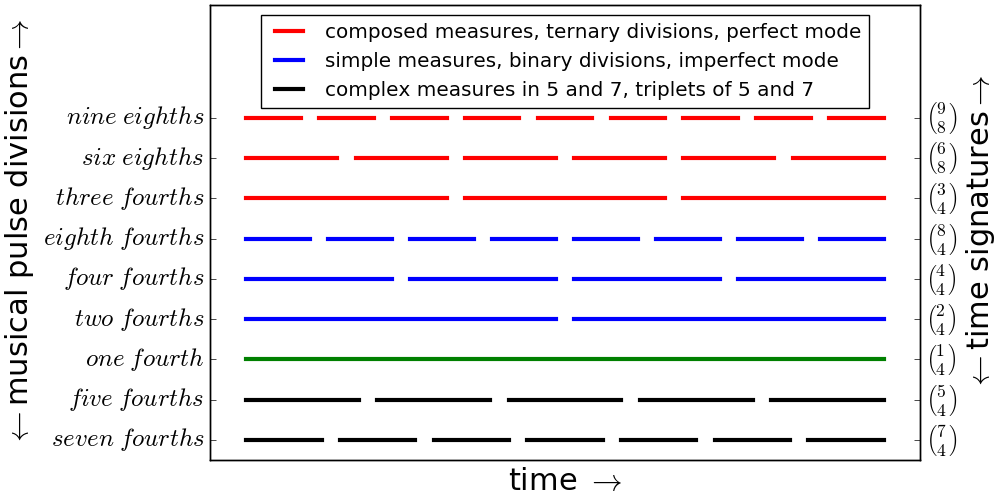
\includegraphics[width=.9\textwidth]{figures/metricaMusical__}
    \caption{Divisions and groupings of the musical pulse for establishing a metric. Divisions of the quarter note, regarded as the
        pulse, is presented on the left. The time signature yield by the corresponding grouping of the music pulse is presented on the right.}
        \label{fig:pulsoSubAgl}
\end{figure*}

Binary divisions are frequent in dance rhythms and celebrations, and are called ``imperfect''.
Ternary relations are typical of
ritualistic and sacred music and are called ``perfect''.
Strong units (accents) fall in the `head' of the units (the first subdivision) and are called downbeats. In binary divisions (2, 4
and 8), strong units alternate with weak units
(e.g.\ division in 4 is: strong, weak, average strong, weak). In ternary divisions
(3, 6 and 9) two weak units succeed the downbeat (e.g.\ division in 3 is:
strong, weak, weak). Division in 6 is considered compound but can also
occur as a binary division. Binary division units which suffer a ternary division yields two units divided into three units each: strong (subdivided in strong,
weak, weak) and weak (also subdivided in strong, weak, weak). Another way to perform
the division in 6 is with a ternary division whose units subdivide as binary,
resulting in: a strong unit (subdivided in strong and weak) and two weak units
(subdivided in strong and weak each).

An accent in the weak beat is a `backbeat', whereas a note starting on a weak beat and persisting across a strong beat is a `syncope'.
These are often found in ethnic and popular music and was used with parsimony in classical music before the XX century.

Notes can occur inside and outside of these divisions of the \emph{'musical metric'}. In most well-behaved cases, notes occur exactly on these divisions, with greater incidence on strong beats.
In extreme cases, rhythmic metric cannot be perceived~\cite{Roederer}. 
Noteworthy is that (usually small or progressive) variations along the temporal grid are crucial for musical interpretation
styles~\cite{Cook}.

Let the pulse be the grouping level $j=0$, the first pulse subdivision be level $j=-1$,
the first pulse agglomeration be level $j=1$ and so on. Accordingly, let $P_i^j$ be the $i$-th unit at grouping level $j$: $P^0_{10}$ is the tenth pulse, $P^{1}_3$ is the third grouped unit (possibly the third measure),
$P^{-1}_2$ is the second part of pulse subdivision. The limits of $j$ are of special interest: pulse divisions are durations perceivable as rhythm; furthermore, the pulses sum, at its maximum, a music or a cohesive set of musical pieces. In other words, a duration given
by $P^{min(j)}_i$, $\forall \; i$, should be greater than $50 ms$ and the durations
summed together $\sum_{\forall i}P^{\text{max}(j)}_i$ should be less than a few
minutes or, at most, a few hours.
These limits might be extrapolated in extreme cases and with aesthetic goals.

Each level $j$ has some parts $i$. When $i$ has three different
values (or multiple of three) there is a perfect (i.e. ternary or compound) relation. When $i$ has only
two, four or eight possible values, than there is an imperfect relation (i.e. binary or simple),
as shown in Figure~\ref{fig:pulsoSubAgl}. Any unit can be
specified as:

\begin{equation}\label{eq:rhythmicUnit}
P^{ \{ j_k \} }_{ \{ i_{k} \}}
\end{equation}

\noindent where $j_k$ is the grouping level and $i_k$ is the unit itself.

As an example, consider $P^{-1,0,1}_{3,2,2}$ as the third subdivision $P^{-1}_3$ of the
second pulse $P^0_2$ and of the second pulse group $P^1_2$ (possibly second measure).
Each unit $P_i^j$ can be associated with a sequence of temporal samples $T$ that constitutes e.g. a
note.
In practice, there is an underlying reference duration, usually associated with the pulse,
e.g. $d_r=1$ second, and the durations of each segment are specified by:
\begin{itemize}
	\item a `temporal notation': where each entry is a relative duration to
		be multiplied by the reference duration. E.g. $durs=\{1,0.5,4\}$
		is mapped to $\{d_id_r\} = \{1d_r, 0.5d_r, 4d_r\}$. Or:
	\item a `frequential notation': where each entry is how many the
		entry that fits a same duration. E.g. $durs=\{4, 2, 16\}$
		is mapped to $\{d_r/d_i\} = \{d_r/4, d_r/2, d_r/16\}$.
		This notation might be less intuitive but it is more tightly
		related to traditional music theory, where e.g. the duration related
		to the number 4 is twice the duration related to the number 8.
\end{itemize}
See the function \texttt{rhythymToDurations} in file \texttt{src/aux/functions.py}
for an implementation of both notations that allows the specification of tuplets
(the use of arbitrary divisions of a reference duration).
The music piece \emph{Poly Hit My} uses different metrics.~\cite{MASSA}

\section{Repetition and variation: motifs and larger units}\label{subsec:motivos}
Given both frequential (chords and scales) and rhythmic (simple, compound and complex beat divisions and agglomerations) musical strata, it is
natural to present them in a coherent and meaningful manner~\cite{Boulez}.
The concept of an arc is essential in this context:
by departing from a context and returning, an arc is made.
One important, and maybe trivial, case is the arc from and to the absence of a unit: from the beginning (unit did not exist before) to the end (unit will not exist from thereon).
The audition of melodic and harmonic lines is permeated by
arcs due to the cognitive nature of the musical hearing: as the mind divides an excerpt, and groups excerpts, each of the units yields an arc.
Accordingly, the note can be considered the smallest (relevant) arc, and each motif and melody as an arc as well.
Each beat and subdivision, each measure and musical
section, constitutes an arc. Music in which the arcs do not present consistency with one another can be understood as music with no coherence. Coherence impression
comes, mostly, from the skilled handling of arcs in a music piece.

Musical arcs are abstract structures and amenable to basic operations. A spectral arc, like a chord, can be inverted, magnified and permuted, to mention just a few possibilities. Temporal arcs, like a melody, a motif, a measure or a note, are also
prone to variations. Let
$S=\left\{s_j=T^j=\{t_i^{j}\}_0^{\Lambda_j-1}\right\}_0^{H-1}$ be a sequence
of $H$ musical events $s_j$, each event with its $\Lambda_j$ samples $t_i^j$
(refer to the Introduction of this Supporting Information document if needed). Bellow is a list of basic techniques
for variation.
\begin{itemize}
        \item Temporal translation is a displacement
    $\delta$ of a specific material to another instant $\Gamma'=\Gamma + \delta$
    of the music. It is a variation that changes temporal localization in
    a music:
    $\left\{s_j'\right\}=\left\{s_j^{\Gamma'}\right\}=\left\{s_j^{\Gamma+\delta}\right\}$
    where $\Gamma$ is the duration between the beginning of the piece (or another reference)
        and the first event $s_0$ of the original structure $S$, and
    $\delta$ is the time offset of the displacement.

    \item Temporal expansion or contraction is a change in duration of each
    arc by a factor $\mu\,:\; s_j'^{\Delta}=s_j^{\mu_j . \Delta}$. Possibly,
    $\mu_j=\mu$ is constant.

    \item Temporal reversion consists on generating a sequence with elements
    in the reverse order of the original sequence $S$, thus: $S'=\left\{s_j'\right\}_0^{H-1}=\left\{s_{(H-j-1)}\right\}_0^{H-1}$.

    \item Pitch translation, or transposition, is a displacement $\tau$ of the pitches.
        It is a variation that changes pitch
        localization:
        $\left\{s_j'\right\}=\left\{s_j^{\Xi'}\right\}=\left\{s_j^{\Xi+\tau}\right\}$
        where $\Xi$ is a reference value, such as the pitch of a section $S$ or of the first event $s_0$.
        If $\tau$ is given in semitones, the transposition displaces a
        frequency $f$ to $\tau_f=f2^{\frac{\tau}{12}}$,
        and the pitch $\Xi_i$ to $\Xi'_i=\Xi_i +12
		\log_2\left(\frac{f'_i}{f_i}\right)$.\footnote{In the MIDI protocol, $\Xi_{f}=55Hz$ when pitch $\Xi=33$
	(an \textit{A1} note). Another good MIDI reference is $\Xi_{f}=440Hz$ and
		$\Xi=69$ (\textit{A4}). The difference ($\Xi_1 - \Xi_2$) is in semitones.
        $\Xi$ is not a measure in semitones: $\Xi=1$ is not a semitone, it is a note with an audible frequency as rhythm, with
		less than 9 periods each second (see Table~\ref{tab:duracoes}).}

        \item Interval inversion is either: 1) the inversion of note pitch order, within the octave equivalence,
            such as described in Section~\ref{subsec:intervalos};
            or 2) the inversion of interval orientation. In the former case, the number of semitones
        is preserved in the ``strict inversion'': $f'_i = 2^{-e} f_i$ where $e$ is a positive constant;
        the inversion is said tonal if the distances are
        considered in terms of the diatonic scale $E_k$:
        $f'_i = f.2^{\left(\frac{12-e_{\left(7-j_e\right)}}{12}\right)}$
        where $j_e$ is the index in $E$ (as in Equation~\ref{eq:relacaoDia}).

        \item Rotation of musical elements is the translation of all elements
        a number of positions ahead or behind, with the care to fill empty positions
        with events which are out of the slots. Thus, a
        rotation of $\tilde{n}$ positions is $s'_n=s_{(n+\tilde{n})\%H}$. If
        $\tilde{n}<0$, it is sufficient to use $\tilde{n}'=H-\tilde{n}$. It is
        usual to associate $\tilde{n}>0$ (events advance) with the clockwise rotation and
        $\tilde{n}<0$ (elements delay) with the anti-clockwise rotation.
        Additional information concerning rotations is given in Section~\ref{estCic}.

        \item The insertion and removal of material in $S$ can be
    ornamental or structural: $S'=\{s_j'\}=\{s_j \text{ if condition A,
    otherwise } r_j\}$, for any $r_j$, including silence.
    Elements can be inserted at the beginning, like a prefix
    for $S$; at the end, as a suffix; or in the middle, splitting $S$ into both
    a prefix and a suffix. Both materials can be mixed in a variety of ways.

    \item Changes in articulation, orchestration and spatialization, or
    $s_j'=s_j^{*_j}$, where $*_j$ is the new characteristic incorporated by 
    element $s_j'$.
    
    \item Accompaniment.
        Musical material presented when $S$ occurs can be modified to yield a variation.
\end{itemize}

From these processes, many others are derived, such as the inverted retrograde, the temporal contraction with an external suffix, etc.
Variations are often thought about in the terms above but are also often very loose,
such as an arbitrary shuffle of the notes in a melody which the composer or performer finds interesting.
As a result, a whole process of mental and neurological activity is unleashed for relating the arcs, responsible for feelings, memories and imaginations, typical of a diligent musical listening.
This cortical activity is critical to
musical therapy, known by its utility in cases of depression and neurological injury.
Also, it is known that regions of the human brain responsible for sonic processing are also used for other activities,
such as for performing verbal discourse and mathematics.~\cite{Sacks,Roederer}

Paradigmatic structures guide the creation of new musical material.
One of the most established structures is the tension/relaxation dipole.
Other traditional dipoles include tonic/dominant, repetition/variation,
consonance/dissonance, coherence/rupture, symmetry/asymmetry,
equivalence/difference, arrival/departure, near/far, and stationary/moving.
All these dipoles are often thought of as parallel or even as equivalent.
Ternary constructions tend to relate to the circle and to unification. The
`transcendental' ternary communion, `modus perfectus', opposes to the `passionate'
dichotomic, `modus imperfectus'~\cite{apel}.
For a scholastic discussion on the composition of motives,
phrases, melodies, themes and musical form (such as rondo, ternary, theme and variations), see~\cite{Schoenberg}.
% melody, answer and reply, motives, etc

\section{Directional structures}\label{subsec:dir}
Musical arcs may be thought of as having two sections: the first reaches the apex and the second returns from apex to the initial region.
This apex is called climax by traditional music theory. It is
usual to distinguish between arcs whose climax is at the beginning, middle, end,
or the first or second half of the duration. These structures are
shown in Figure~\ref{fig:climax}. The varying parameter can be non-existent, a case in which
the arc consists only of a reference structure, a case which resembles a note without the fundamental frequency.~\cite{Schoenberg}

\begin{figure}
    \centering
        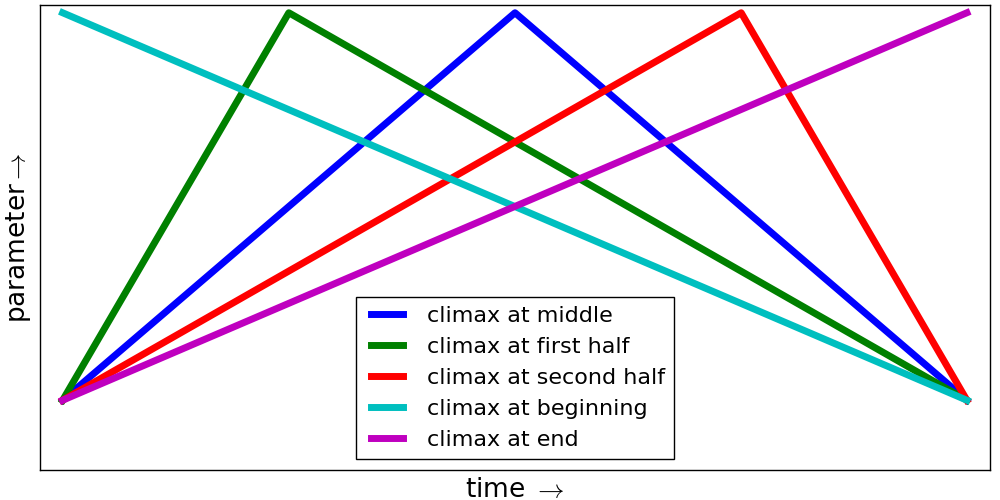
\includegraphics[width=.8\columnwidth]{figures/climax_}
        \caption{Canonical distinctions of musical climax in a given melody and
        other arcs. The possibilities considered are: climax at the beginning, at the first half, in the middle, in the second half and 
        at the end. The x and y-axis parameters can be non-existent and yield only a reference structure.}
        \label{fig:climax}
\end{figure}

Consider the sequence $S=\{s_i\}_0^{H-1}$ with a monotonic variation of a characteristic.
The sequence
$R=\{r_i\}_0^{2H -2}=\left\{s_{(H-1-|H-1-i|)}\right\}_0^{2H-2}$
presents perfect specular symmetry, i.e.\ the second half is the
mirrored version of the first. In musical terms, the climax is
in the middle of the sequence. It is possible to achieve different results
by using sequences with different sizes. All the mathematics of
sequences, already well established and taught routinely in calculus courses, can be used to generate these arcs~\cite{Guidorizzo,Schoenberg}.
Theoretically, when applied to any characteristic of musical events,
these sequences produce arcs, since they imply a deviation and return of an initial context (parametrization, state, etc).
Henceforth, it is possible for a given sequence to have
numerous distinct arcs, with different sizes and climaxes. 
This is an interesting and useful resort, and the correlation of arcs yields coherence~\cite{Salzer}.

In practice, and historically, there is special incidence and use of the golden ratio.
The Fibonacci sequence might be generalized as follows in order for any two numbers to be used
and approximate the golden ratio.
Given any two numbers $x_0$
and $x_1$, define the elements of the sequence $\{x_n\}$ as: $x_n=x_{n-1}+x_{n-2}$.
The greater $n$ is, the more $\frac{x_{n}}{x_{n_1}}$ approaches the golden ratio
($1.61803398875...$). The sequence converges fast even with discrepant
initial values.
E.g. let $x_0=1$, $x_1=100$ and $y_n=\frac{x_n}{x_{n+1}}$, the error for the first values with
respect to the golden ratio is, approximately, $\{ e_n \}
=\left\{100\frac{y_n}{1.61803398875}-100 \right\}_1^{10}=\{6080.33, -37.57, 23,
-7.14, 2.937, -1.09, 0.42, -0.1601, 0.06125, -0.02338\}$. The Fibonacci sequence
presents the same error progression, but starts at the second step of a more discrepant initial setting
($\frac{1}{1}\approx\frac{100+1 = 101}{100}$).
One might benefit from the On-Line Encyclopedia of Integer Sequences (OEIS~\cite{oeis})
for exploring various sequences.

The musical piece \emph{Dirracional} exposes the use of arcs in explicit directional structures.~\cite{MASSA}

\section{Cyclic structures}\label{estCic}
The philosophical understanding that human thought is founded on the recognition of similarities and differences (e.g. as perceived in stimuli), places symmetries
at the core of cognition~\cite{Deleuze}.
Mathematically, it is commonplace to express symmetries as algebraic groups, and a finite group is always isomorphic to a permutation
group (by Cayley's theorem).
In a way, this states that permutations can express any symmetry in a
finite system~\cite{gruposFascination}.
Also, any permutation set can be used as a generator of an algebraic group~\cite{permMusic}.
In music, permutations are ubiquitous in scholastic techniques,
 which confirms their central role.
The successive application of permutations generates cyclic arcs~\cite{change,Zamacois,permMusic} and
e.g. these two academic documents report on the generation of musical structures using permutation groups:~\cite{figgusOriginal, figgusEspacializacao}.
The properties defining a group $G$ are:

\begin{equation}\label{eq:groups}
\begin{split}
\forall \;\; p_1,p_2 \in G \Rightarrow  \quad   & p_1 \bullet p_2  = p_3 \in G \\ 
     & \text{(closure property)} \\
\forall \;\; p_1,p_2,p_3 \in G \Rightarrow \quad & (p_1\bullet p_2)\bullet p_3  = p_1\bullet (p_2\bullet p_3) \\
     & \text{(associativity property)} \\
\exists \;\; e \in G :                  \quad    & p \bullet e  = e \bullet p \;,\;\;\; \forall\; p \in G  \\ 
     &  \text{(existence of the identity element)} \\
\forall \;\; p \in G, \;\exists\; p^{-1} :\quad  &  p\bullet p^{-1}i =p^{-1}\bullet p = e \\
     &  \text{(existence of the inverse element)}
\end{split}
\end{equation}

From the first property follows that two permutations act as one permutation. In fact, it is possible to apply a
permutation $p_1$ and another permutation $p_2$, and, comparing both initial and final orderings, observe another permutation $p_3$.
Every element $p$ operated with itself a sufficient number of times $n$ reaches the identity element $p^n=e$ (otherwise the group generated by $p$ would be infinite).
The order $n$ of an element $p$ is
the lowest $n\,:\;p^n=e$.
Thus, a finite
permutation $p$, successively applied, reaches the initial ordering of its
elements, and yields a cycle. This cycle, if used for parameters of notes or other musical structures,
yields a cyclic arc.

These arcs can be established by using one or a set of permutations.
As a historical
example, the \emph{change ringing} tradition conceives music through
bells played one after another and then played again, but in a different
order. This process is repeated until it reaches the initial ordering. The sequence of
different orderings is a \emph{peal}. Table~\ref{tab:change}
presents a traditional \emph{peal}, named ``Plain Change''~\cite{change}, for 3 bells (\textcolor{red}{1}, \textcolor{blue}{2} and \textcolor{green}{3}), which explores
all possible orderings. Each line indicates one bell ordering to be
played. Permutations occur between each line. In this case, the musical structure
consists of permutations that entail a cyclic behavior.

\begin{table}[htp!]
\centering
\caption{Change Ringing: a traditional \emph{peal} for 3 bells. Permutations
occur between each line. Each line is a bell ordering and each ordering is played at a time.} 
\begin{tabular}{l c r}
\textcolor{red}{1} & \textcolor{blue}{2} & \textcolor{green}{3} \\
\textcolor{blue}{2} & \textcolor{red}{1} & \textcolor{green}{3} \\
\textcolor{blue}{2} & \textcolor{green}{3} & \textcolor{red}{1} \\
\textcolor{green}{3} & \textcolor{blue}{2} & \textcolor{red}{1} \\
\textcolor{green}{3} & \textcolor{red}{1} & \textcolor{blue}{2} \\
\textcolor{red}{1} & \textcolor{green}{3} & \textcolor{blue}{2} \\
\textcolor{red}{1} & \textcolor{blue}{2} & \textcolor{green}{3}
\end{tabular}
\label{tab:change}
\end{table}

The use of permutations in music can be summarized in the following way:
let $S=\{s_i\}$ be a sequence of musical events $s_i$ (e.g.\ notes), and $p$ a
permutation. $S'=p(S_i)$ comprises the same elements of $S$ but in a
different order. Permutations have two notations: cyclic and
natural. The natural notation basically indicates the original indexes in the order that results from
the permutation. Thus, given the original ordering of the sequence by its indexes $[0\;1\;2\;3\;4\;5\;...]$, the permutation is noted by the sequence of indexes it
produces (e.g. $[1\;3\;7\;0\;...]$).
In the cyclic notation, a permutation is expressed
by swaps of elements and its successors.
E.g. $(1,2,5)(3,4)$ in cyclic notation is equivalent to $[0,2,5,4,3,1]$ in natural notation.

In the auralization of a permutation, it is not necessary to permute elements of $S$,
but only some characteristic. Thus, if $p$ is a permutation and $S$ is a sequence of basic notes as in the end of Section~\ref{notaBasica}, the
sequence $S'=p^f(S)=\left\{s_i^{p(f)}\right\}$ consists of the same
musical notes, following the same order and maintaining the same characteristics, but with the
fundamental frequencies permuted according to $p$.

Two subtleties of this procedure should be commented upon. 
First, a permutation $p$ is not restricted to involve all elements of $S$, i.e.\ it can operate in a subset of $S$.
Second, not all elements $s_i$ need to be executed at each access to $S$.
To exemplify, let $S$ be a sequence of music notes $s_i$. 
If $i$ goes from $0$ to $n$, and
$n>4$, at each sequence of $4$ notes it is possible to execute e.g. only the first $4$
notes.
The other notes of $S$ can occur in other events where permutations 
allocate such notes to the first four events.
The execution of disjoint sets of $S$
is the same as modifying the permutation and executing the first $n$ notes.

In summary, to each permutation $p$, we have to determine:
1) note characteristics where it operates (frequency, duration, \emph{fades},
intensity, timbre, etc); and
2) the period of incidence (how many times $S$ is used before a permutation is
applied).

The PPEPPS/FIGGS and the \emph{3 Trios} present respectively a computational implementation
and an instrumental musical piece that use
permutations to achieve
musical structures~\cite{MASSA,figgusOriginal,figgusEspacializacao,figgus,3Trios}.

\section{Serialism and post-serial techniques}
Recapitulating concepts from Sections~\ref{sec:atonal} and~\ref{subsec:motivos},
sequences of characteristics can be predefined and
used throughout a musical piece.
These sequences can be of intensities, timbre, durations,
density of events, etc.
Sequences can be used very strictly or loosely,
such as by skipping some elements.
The sequences can be of different sizes, yielding arcs
until the initial condition is reached again (i.e. cycles as in Section~\ref{estCic}).
One paradigmatic case is the ``total serialism'' where all
the musical characteristics are serialized~\cite{Lovelock}.
Although the use of sequences is inherent to music (e.g. scales, metric pulses),
their use with greater emphasis than tonal (or modal) elements
in western music, as an artistic trend, took place only in the
first half of the twentieth century and is called ``serialism''.
Post-serial techniques are numerous, and brief descriptions of
important concepts to exemplify them are:
\begin{itemize}
	\item Spectralism:
		consists on the use the (Fourier) spectrum of a sound or the harmonic series for musical composition,
		such as
		to obtain harmonies, sequences of pitches or a temporal evolution of the overall spectrum.
		For example, the most prominent frequencies can be used as pitches,
		real notes can be used to mimic an original spectrum
		(e.g. use piano notes to mimic the spectrum of a spoken sentence) or portions of the spectrum made to vary.~\cite{grisey}
	\item Spectromorphology:
		can be considered a spectral music (spectralism) theoretical framework~\cite{smalley,schaeffer}
		that examines the relation between sound spectra and their temporal evolution.
		The theory poses e.g. different onsets, continuations and terminations; characteristics of (sonic) ``motion'';
		and spectral density.
	\item Stochastic music:
		the use of random variables to describe musical elements are extensively considered in stochastic music~\cite{formalized}.
		In summary, one can use probability distributions for the synthesis of basic sounds and for obtaining larger scale musical structures.
		Changes in these distributions or in other characteristics yield the discourse.
	\item Textures:
		sounds may be assembled in terms of a ``sonic texture''.
		Sonic textures are often thought about very abstractly
		as a sonic counterpart of visual textures.
		Examples of parameters that are used: range between highest and lowest note,
		density of notes, durations of notes, motives, number of voices.
		If the sounds are small enough (typically $<$ $100ms$) the process can be though of in terms of \emph{granular synthesis}~\cite{microsound}.
\end{itemize}

\section{Musical idiom?}
In numerous studies and aesthetic endeavors, there are models, discussions and exploitation of a `musical language'.
Some of them are linguistic theories applied to music
and some discern different `musical
idioms'~\cite{Lerdahl, Harmonia, Salzer,Alfaix}. Simply put, a musical idiom or language
is the result of chosen materials together with variation techniques and
relations established between elements along a music piece. In these matters,
dichotomies are prominent, as explained in Section~\ref{subsec:motivos}:
repetition and variation, relaxation and tension, stability and instability, consonance and dissonance, etc.
A thorough discussion of what can be considered a musical language is out of the scope of this article, but this brief consideration of the subject is useful as a convergence of all the previous content.

\section{Musical usages}\label{subsec:usosmusicais3}
The basic note was defined and characterized in quantitative terms in Section~\ref{sec:notaDisc}.
Next, the internal note
composition was addressed within both internal transitions and elementary sonic treatment
(Section~\ref{sec:varInternas}). Finally, this section aims at organizing these notes in music. The numerous resources and consequent infinitude
of praxis possibilities is typical and highly relevant for artistic contexts~\cite{Harmonia,Webern}.

There are studies and further developments for each of the presented resources.
For example, it is possible to obtain `dirty' triadic harmonies (with notes out of the triad) by superposition of perfect fourths.
Another interesting example is the superimposition of rhythms in different metrics, constituting what is
called \emph{polyrhythm}. The music piece \emph{Poli-hit my}~\cite{MASSA} explores these simultaneous metrics by impulse trains convolved with notes.

Microtonal scales are important for 20th
century music~\cite{microtonalidade} and yielded diverse remarkable results throughout history, e.g.
fourths of a tone ($\epsilon=2^{\frac{1}{24}}$) are often used in some genres of Indian and Arabic music.
The musical sequence \emph{MicroTone}~\cite{MASSA} explores these possibilities,
including microtonal melodies and harmonies
with many pitches in a very reduced frequency bandwidth.

As in Section~\ref{subsec:mus2}, relations between
parameters are powerful to achieve musical pieces.
E.g. the number of permuted
notes can vary during the music, a relationship between permutations and the piece
duration. Harmonies can be obtained from triads (Equations~\ref{triades}) with duplicated
notes at each octave and more numerous duplication when the depth and frequency of
vibratos are lower (Equations~\ref{vbrGamma},~\ref{vbrAux},~\ref{vbrF},~\ref{vbrGamma2},~\ref{vbrT}).
Incontestably, the possibilities are very wide, which is made evident by the numerous musical pieces and styles.

The symmetries at octave divisions (Equations~\ref{escSim}) and the
symmetries presented as permutations (Table~\ref{tab:change} and
Equations~\ref{eq:groups}) can be used together. In the music piece \emph{3 trios},
this association is performed in a systematic way in order to achieve a specific style.
This is an instrumental piece, not included as a source code but available online~\cite{3Trios}.
\emph{PPEPPS} (Pure Python EP: Project Solvent) is an EP (Extended Play) synthesized using
resources presented in this document. With minimal parametrization, the scripts
generate complete musical pieces, allowing easy composition of sets of
music.~\cite{figgus} A simple script of a few lines specifies music delivered as 16 bit
44.1kHz PCM files (WAVE). This facility and technological
arrangement creates aesthetic possibilities for both sharing and education.
The Half-Shape Suite consists in a collection of pieces elaborated around the ideas of symmetries on sets of small cardinalities (i.e. number of elements), composed and synthesized using the MASS framework, the ``music'' package, and found in the \texttt{/src/finalPiece/} directory.~\cite{MASSA,music,halfSuite}

% \bibliography{sample-bibliography}
\bibliographystyle{ACM-Reference-Format}
\bibliography{./article2}
\end{document}
